\documentclass[12pt,a4paper]{article}
\usepackage[UTF8]{ctex}
\usepackage{graphicx}
\usepackage{geometry}
\usepackage{ulem}
\usepackage{enumitem}
\usepackage{titlesec}
\usepackage{multicol}
\usepackage[export]{adjustbox}
\usepackage{amsmath}  % 推荐用于更好的数学排版
\usepackage[utf8]{inputenc}
\usepackage{CJKutf8}
\usepackage{fancyhdr}
\usepackage{lastpage}
\usepackage{ulem}
\usepackage{tabularx}
\usepackage{float}
\usepackage{siunitx}
\usepackage{multirow} 
\usepackage{tikz}
\usepackage{listings}
\usepackage{xcolor}
\usepackage{circuitikz} 
\usetikzlibrary{shapes,arrows,positioning}


\lstset{
    language=C++,
    basicstyle=\small\ttfamily,
    keywordstyle=\color{blue},
    commentstyle=\color{green!60!black},
    stringstyle=\color{red},
    numbers=left,
    numberstyle=\tiny\color{gray},
    frame=single,
    breaklines=true,
    tabsize=2
}


% 页眉页脚设置
\pagestyle{fancy}
\fancyhf{} % 清除所有页眉页脚
% 设置页眉内容
%-==========1. 填写从第二页开始 每页第一行的信息==========-
\fancyhead[C]{\small
    \makebox[4.5em][c]{实验名称：} \uline{\makebox[17em][c]{Arduino多功能数字时钟}} 
    \makebox[2.5em][c]{姓名：} \uline{\makebox[4em][c]{张赫}} 
    \makebox[2.5em][c]{学号：} \uline{\makebox[5em][c]{3240101459}}
}%--------------------------------------------------------
\fancyfoot[C]{\small 第 \thepage\ 页，共 \pageref{LastPage} 页}


% 取消页眉和页脚的下划线
\renewcommand{\headrulewidth}{0pt} % 页眉横线粗细设为0
\renewcommand{\footrulewidth}{0pt} % 页脚横线粗细设为0

% 调整页眉高度
\setlength{\headheight}{50pt}

% 设置plain样式（用于第一页）
\fancypagestyle{plain}{
    \fancyhf{} % 清除所有页眉页脚
    \renewcommand{\headrulewidth}{0pt} % 隐藏页眉横线
    \fancyfoot[C]{第 \thepage\ 页，共 \pageref{LastPage} 页} % 保留页脚
}
% 设置页面边距
\geometry{left=2.54cm,right=1.5cm,top=2.54cm,bottom=2.54cm}

% 设置正文字体大小为小四
\renewcommand{\normalsize}{\fontsize{12pt}{16pt}\selectfont}
% 设置章节格式
\titleformat{\section}{\fontsize{16pt}{22pt}\selectfont\bfseries}{\thesection}{1em}{} % 一级标题：三号
\titleformat{\subsection}{\fontsize{15pt}{20pt}\selectfont\bfseries}{\thesubsection}{1em}{} % 二级标题：小三

\begin{document}
\thispagestyle{plain}%第一页使用 plain 样式，而不是默认的 fancy 样式，第一页不再显示页眉
% 标题部分 - 两栏布局
\begin{multicols}{2}
    % 左栏：图片和实验报告标题
    % 左栏：使用空行创建前三行
    \noindent
    ~\\ % 第一行
    ~\\ % 第二行
    ~\\ % 第三行
    \hphantom{占位}% 使用空占位符
    \raisebox{-0.5\baselineskip}% 图片向下移动半行
    {
\includegraphics[width=1.85in,height=0.58in]{ZJU.jpg}}
    \hspace{.5em}% 图片和标题之间的间距
    \raisebox{0pt}[\height][0pt]% 标题底部对齐
    {\textbf{\fontsize{26pt}{30pt}\selectfont 实验报告}}
    
    \columnbreak % 换到右栏
    
    % 右栏：个人信息
    % 右栏：个人信息 - 靠右对齐 
%-==========2. 填写个人信息==========-
    \begin{flushright}
        \small

        \makebox[3em][l]{专业：} \uline{\makebox[9em][c]{法语-电子科学与技术}} \\
        \makebox[3em][l]{姓名：} \uline{\makebox[9em][c]{张赫}} \\
        \makebox[3em][l]{学号：} \uline{\makebox[9em][c]{3240101459}} \\
        \makebox[3em][l]{日期：} \uline{\makebox[9em][c]{2026年5月13日}} \\
        \makebox[3em][l]{地点：} \uline{\makebox[9em][c]{紫金港东四216}} \\
    \end{flushright}   
\end{multicols}
% 课程名称等信息（单栏）
%-==========3. 填写课程信息==========-

{\small
\noindent
课程名称： \uline{电子电路设计实验II} \hfill 指导老师： \uline{施红军、叶险峰、邓靖靖} \hfill 成绩： \uline{\hspace{3cm}} \\
实验名称：\uline{Arduino多功能数字时钟}\hfill 实验类型：\uline{设计实验}\hfill 同组学生姓名：\uline{虞悦}
}
%-==========4. 正文开始==========-

\section*{零、示例项目}

设计电流-电压转换电路，将 4-20mA 标准电流信号转换为 0-10V 的标准电压信号。
\subsection*{0.1 原理图}

\begin{figure}[H]
    \centering
    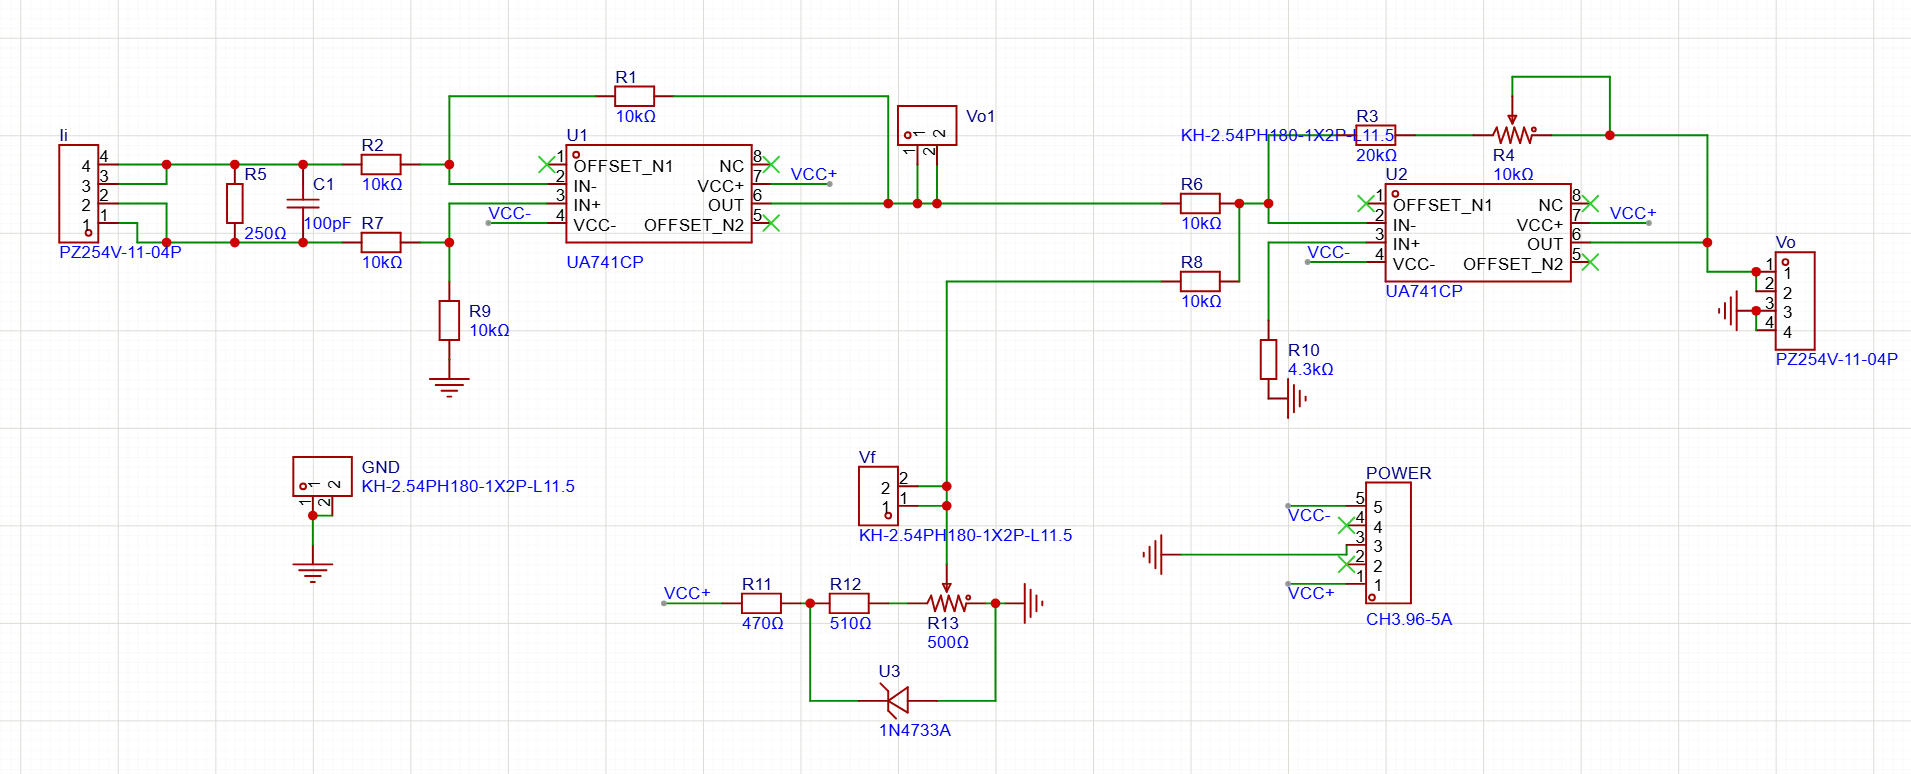
\includegraphics[width=1\textwidth]{A0.png}
    \caption{原理图}
\end{figure}

变送器输出的 \(4\sim20\,\text{mA}\) 标准电流信号需转换为 \(0\sim10\,\text{V}\) 电压信号。
其中：
\[
4\,\text{mA} \rightarrow 0\,\text{V},\quad
12\,\text{mA} \rightarrow 5\,\text{V},\quad
20\,\text{mA} \rightarrow 10\,\text{V}.
\]

\subsubsection*{第一级：电流取样与差动放大}
电阻 \(R_1\) 跨接在电流源两端，对输入电流 \(I_i\) 取样。运放 \(A_1\) 与 \(R_2, R_3, R_4, R_5\) 构成差动放大器。
若 \(R_2 = R_3 = R_4 = R_5\)，则：
\[
V_{o1} = -I_i R_1.
\]

\subsubsection*{第二级：反相加法器}
第二级为反相加法器，实现电平变换：
\[
V_o = -\frac{R_f}{R_6} V_{o1} - \frac{R_f}{R_7} V_f 
     = \frac{R_f}{R_6} I_i R_1 - \frac{R_f}{R_7} V_f.
\]
合理选择 \(R_6, R_7, R_f, V_f\)，可使 \(I_i\) 从 \(4\,\text{mA}\) 到 \(20\,\text{mA}\) 变化时，
\(V_o\) 从 \(0\,\text{V}\) 到 \(10\,\text{V}\) 线性变化。

\subsubsection*{\(V_f\) 稳压电路}
为使 \(V_f\) 不受电源电压波动影响，采用 \(5.1\,\text{V}\) 稳压管构成稳压电路，经分压后产生所需的可调 \(V_f\)。

\subsection*{0.2 PCB设计}

\begin{figure}[H]
    \centering
    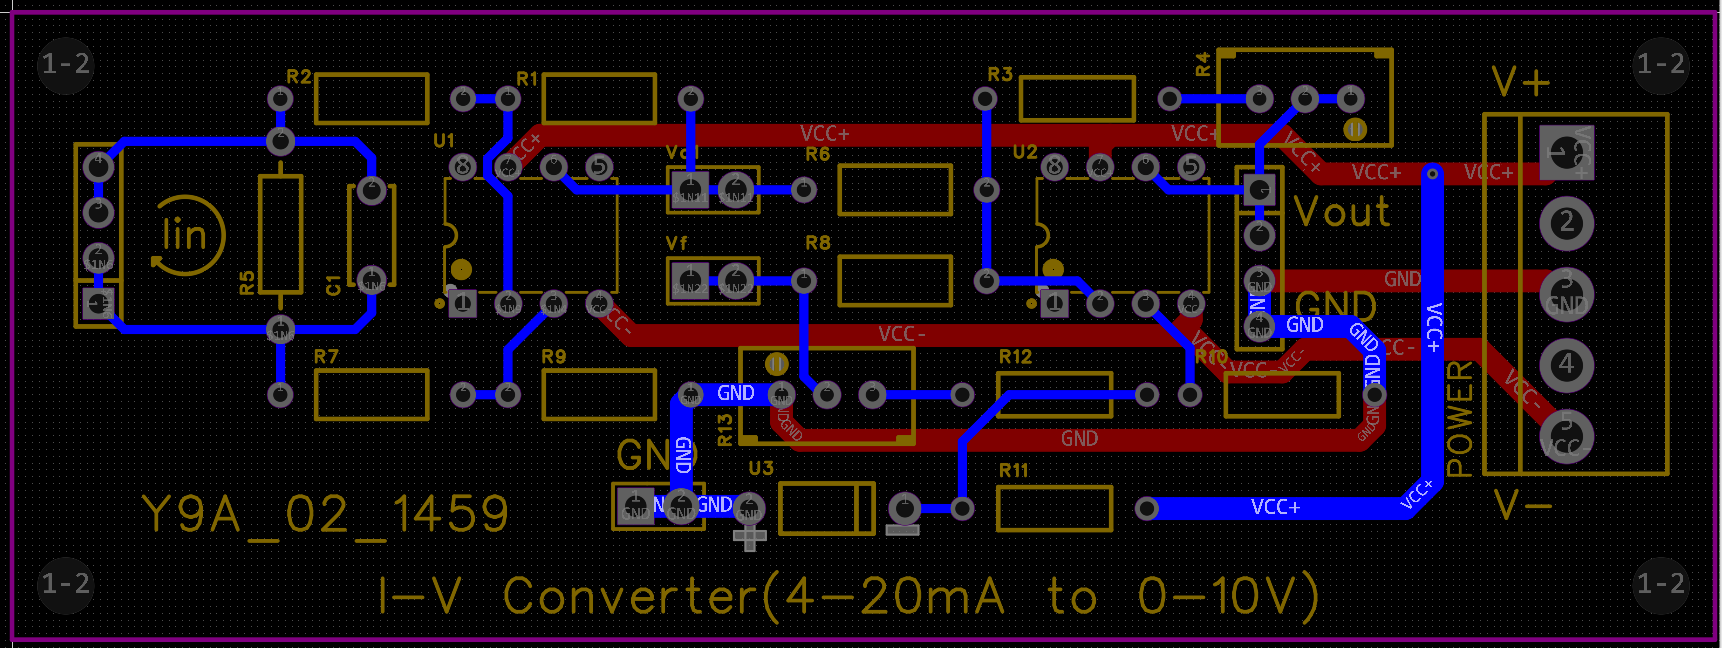
\includegraphics[width=0.8\textwidth]{A1.png}
    \caption{PCB设计}
\end{figure}

\subsection*{0.3 实验数据记录}

焊接完成后进行调试，得到以下数据：

\begin{table}[H]
\centering
\begin{tabular}{|c|c|}
    \hline
    输入电流（mA） & 输出电压（V） \\
    \hline
    4 & -46.104mV \\
    \hline
    8 & 2.4632 \\
    \hline
    12 & 4.9765 \\
    \hline
    16 & 7.4877 \\

    \hline
    20 & 10.001 \\
    \hline

    
\end{tabular}
\caption{实验数据记录}
\end{table}
从数据可以看出，输出电压与输入电流呈线性关系，且完全符合实验要求。

\section*{一、实验目的}

1、掌握 Arduino 平台的基本使用方法，包括硬件连接、编程环境配置及代码编写。

2、了解数字时钟的基本原理，学会如何设计并制作一个多功能数字时钟。

3、能够独立完成一个基于 Arduino 的多功能数字时钟项目的设计、制作与调试。


\section*{二、实验任务与要求}


1、设计并制作一个能够显示时间、日期和星期的多功能数字时钟。

2、实现闹钟功能，当达到设定时间时，能够通过蜂鸣器或 LED 进行提示。

3、（可选）实现温度显示功能，通过温度传感器实时显示当前环境温度。

4、编写相应的 Arduino 程序，实现数字时钟的各项功能。

\section*{三、实验原理}

本节将详细介绍实验中各个核心模块的工作原理，包括实时时钟模块、显示模块、编码器输入模块、音频播放模块以及各类传感器模块。

\subsection*{3.1 DS3231实时时钟模块}

DS3231是一款高精度I2C实时时钟芯片，内置温度补偿晶体振荡器（TCXO）和晶体谐振器。其核心工作原理如下：

\begin{figure}[H]
    \centering
    
\includegraphics[width=0.6\textwidth]{1.png}
    \caption{DS3231实时时钟模块}

    
\end{figure}

\begin{figure}[H]
    \centering
    
\includegraphics[width=0.6\textwidth]{2.png}
    \caption{DS3231时钟芯片原理图}
    \end{figure}



\subsubsection*{时钟计时}

DS3231内部包含一个秒、分、时、日、月、年寄存器，采用BCD码格式存储时间数据。芯片上电后自动从备用电池取电，保持计时连续性。计时精度主要依赖于内部32.768kHz石英晶体的振动频率。
\begin{equation}
f_{osc} = 32768 \text{ Hz} = 2^{15} \text{ Hz}
\end{equation}

通过15级二分频电路，将32.768kHz的频率精确分频为1Hz的秒脉冲，驱动计时器递增。

\subsubsection*{温度补偿机制}

DS3231内部集成温度传感器，每64秒进行一次温度测量，根据实测温度动态调整晶体振荡器的负载电容，从而补偿温度变化引起的频率漂移。补偿后的精度为
$2\text{ppm} \quad (-40^\circ\text{C} \text{ 至 } +85^\circ\text{C})$，每月误差不超过$\pm 5.2$秒。


\subsection*{3.2 1.8寸TFT显示屏（ST7735）}

本次实验使用一块1.8寸的TFT显示屏作为显示模块，驱动芯片为ST7735。此芯片在Arduino IDE上有现成的库可以驱动。

\begin{figure}[H]
    \centering
    
\includegraphics[width=0.4\textwidth]{3.jpg}
    \caption{1.8寸TFT显示屏}

\end{figure}

ST7735是一款支持SPI接口的TFT-LCD驱动芯片，分辨率可达128×160像素，支持262K色显示。

\subsubsection*{显示原理}

TFT（Thin Film Transistor）液晶显示屏每个像素点对应一个薄膜晶体管，通过控制液晶分子的偏转角度来调节背光的透过率，从而实现不同灰阶和颜色的显示。ST7735内部集成GRAM（图形RAM），存储待显示的图像数据。

\subsubsection*{SPI通信协议}

显示屏通过SPI总线与主控通信，引脚功能如下：

\begin{table}[H]
\centering
\begin{tabular}{|c|c|c|}
\hline
\textbf{引脚} & \textbf{方向} & \textbf{功能说明} \\
\hline
SCL & 输入 & SPI时钟信号 \\
\hline
SDA & 输入 & SPI数据信号 \\
\hline
CS & 输入 & 片选信号（低电平有效） \\
\hline
DC & 输入 & 数据/命令选择（高电平：数据，低电平：命令） \\
\hline
RES & 输入 & 复位信号（低电平有效） \\
\hline
\end{tabular}
\caption{ST7735 SPI引脚功能}
\end{table}


\subsection*{3.3 EC11旋转编码器}

EC11编码器是一种增量式光电/机械编码器，通过检测A、B两相输出的相位差来判断旋转方向和步数。

\subsubsection*{工作原理}

编码器内部有两个光耦或机械触点，旋转时输出两路相位差$90^\circ$的方波信号：

\begin{figure}[H]
\centering

\includegraphics[width=0.6\textwidth]{4.png}
\caption{编码器输出波形}
\end{figure}

当顺时针旋转时，A相领先B相$90^\circ$；逆时针旋转时，B相领先A相$90^\circ$。通过检测A相下降沿时的B相电平即可判断方向：

\begin{equation}
\text{方向} = 
\begin{cases}
\text{顺时针} & \text{if } (A\downarrow \text{ 且 } B = \text{HIGH}) \\
\text{逆时针} & \text{if } (A\downarrow \text{ 且 } B = \text{LOW})
\end{cases}
\end{equation}



\subsection*{3.4 DFPlayer Mini音频模块}

DFPlayer Mini是一款支持MP3/WAV格式解码的串口控制音频模块，集成了MicroSD卡槽和3W功放。


\begin{figure}[H]
    \centering
    
\includegraphics[width=0.2\textwidth]{5.jpg}
    \caption{DFPlayer Mini音频模块}

    
\end{figure}
\subsubsection*{解码原理}

模块内部采用专用音频解码芯片，读取SD卡中的MP3文件后，经过以下处理流程：

\begin{enumerate}
    \item 位流解复用：解析MP3帧头信息
    \item 霍夫曼解码：还原量化后的频域系数
    \item 逆量化：恢复真实的频域幅度值
    \item IMDCT变换：将频域信号转换回时域PCM信号
    \item 合成滤波：输出连续音频波形
\end{enumerate}

\subsubsection*{串口控制协议}

通过软串口发送指令控制播放功能，指令格式为：

\begin{table}[H]
\centering
\begin{tabular}{|c|c|c|c|c|c|c|}
\hline
起始字节 & 版本号 & 数据长度 & 指令码 & 反馈标志 & 参数高字节 & 参数低字节 \\
\hline
0x7E & 0xFF & 0x06 & CMD & 0x00 & DataH & DataL \\
\hline
\end{tabular}
\caption{DFPlayer指令帧格式}
\end{table}

常用指令示例：
\begin{itemize}
    \item 播放指定曲目：0x03 + 曲目号
    \item 调节音量：0x06 + 音量值(0-30)
    \item 停止播放：0x16
\end{itemize}

\subsection*{3.5 DHT11温湿度传感器}

DHT11采用单总线通信协议，内部包含一个电阻式湿度传感器和NTC温度传感器。


\subsubsection*{单总线通信协议}

通信时序如图\ref{fig:dht11}所示：

\begin{figure}[H]
\centering


\includegraphics[width=1\textwidth]{6.png}
\caption{DHT11通信时序图}
\label{fig:dht11}
\end{figure}

数据传输长度为40位，格式为：
\begin{equation}
\text{8位湿度整数} + \text{8位湿度小数} + \text{8位温度整数} + \text{8位温度小数} + \text{8位校验和}
\end{equation}

\subsection*{3.6 光敏传感器}

数字输出型光敏传感器模块主要由光敏电阻和电压比较器组成。

\begin{figure}[H]
    \centering
    
\includegraphics[width=0.8\textwidth]{7.jpg}
    \caption{光敏传感器模块原理图}
    \end{figure}

\subsubsection*{比较器阈值判断}

传感器模块将光敏电阻与固定电阻分压后输入电压比较器，当照度超过设定阈值时，数字输出引脚电平翻转：

\begin{equation}
V_{out} = 
\begin{cases}
\text{LOW} & \text{if } V_{LDR} > V_{ref} \\
\text{HIGH} & \text{if } V_{LDR} < V_{ref}
\end{cases}
\end{equation}


本实验利用该特性实现环境光检测，从而自动切换屏幕配色方案。


\section*{四、实验设计}


\subsection*{4.1 功能设计}

本节阐述系统设计前期的功能构思，明确智能闹钟应具备的核心功能与用户需求。

\subsubsection*{功能需求概述}

本系统旨在设计一款集时间显示、闹钟提醒、环境监测于一体的智能闹钟，满足用户对时间管理的基础需求。

\subsubsection*{时钟显示功能}

系统可支持两种时钟显示方式，用户可根据喜好自由切换：
\begin{itemize}
    \item \textbf{数字时钟模式}：以数字形式显示时、分、秒及完整日期
    \item \textbf{模拟时钟模式}：以表盘形式显示时间，包含时、分、秒指针
\end{itemize}

同时，时钟时间应与RTC模块保持实时同步，确保计时精度。

\subsubsection*{闹钟管理功能}

系统支持设置多组独立闹钟，满足用户不同时间段的提醒需求。每组闹钟具备独立的启用/禁用开关，用户可根据需要灵活控制。闹钟在当天触发过一次后不再重复响铃，次日自动重置，避免同一闹钟反复响起。

\subsubsection*{环境监测功能}

实时采集环境温度并显示，帮助用户了解当前室温状况；实时采集环境湿度并显示，提供环境舒适度参考。

\subsubsection*{交互控制功能}

采用单编码器实现全部人机交互，包括：
\begin{itemize}
    \item 旋转操作：用于数值调整和选项切换
    \item 短按操作：用于确认和字段切换
    \item 长按操作：用于模式切换
\end{itemize}
系统支持在时钟显示和闹钟设置两种模式之间切换。

\subsubsection*{闹钟触发响应}
闹钟触发时系统应执行以下动作：
\begin{itemize}
    \item 播放预设的MP3提示音
    \item 输出控制信号供外部设备使用
    \item 屏幕显示醒目的闹钟提示
    \item 响铃持续一段时间后自动停止
\end{itemize}

\subsubsection*{主题自动切换}
系统应能检测环境光线强度，根据光照条件自动切换屏幕配色方案（深色/浅色），提升不同环境下的观看体验。



\subsubsection*{功能优先级}

根据用户日常使用需求，将各项功能划分为三个优先级等级：

\begin{table}[H]
\centering
\begin{tabular}{|c|c|l|}
\hline
\textbf{优先级} & \textbf{功能类别} & \textbf{具体功能} \\
\hline
\textcolor{red}{高} & 时钟显示 & 数字/模拟双模式时间显示 \\
\hline
\textcolor{red}{高} & 闹钟管理 & 闹钟触发与响铃 \\
\hline
\textcolor{orange}{中} & 闹钟管理 & 多组闹钟设置与开关 \\
\hline
\textcolor{orange}{中} & 交互控制 & 编码器操作与模式切换 \\
\hline
\textcolor{green}{低} & 环境监测 & 温湿度检测与显示 \\
\hline
\textcolor{green}{低} & 智能响应 & 主题自动切换 \\
\hline
\end{tabular}
\caption{功能优先级分级}
\end{table}

\subsection*{4.2 模块选择}

\subsubsection*{显示模块}
显示模块可以选择LCD1602、OLED或者TFT-LCD。

LCD1602只能显示数字、英文、且输出的容量有限，不能显示复杂图形。

OLED模块使用I2C通讯，常见的0.96寸/1.3寸分辨率为128x64，可显示复杂图形。但是只能单色显示，虽然也有双色模块但是固定第一行黄色，第二至四行蓝色的模式。

TFT-LCD模块使用SPI通讯，常见的1.8寸分辨率为128x160，支持全彩显示。

为了让时钟有良好的观感，本次实验我们选用TFT-LCD显示屏作为显示模块。

\subsubsection*{用户输入}

用户输入可以选择开关、按键或编码器等。

开关可以方便地实现简单功能，如开关闹钟、开关显示模式。

按键可以方便地实现复杂功能，如按键切换闹钟、按键设置闹钟。

编码器可以实现全部人机交互，包括旋转操作、短按操作、长按操作。

为了实现全部人机交互，本次实验我们选用编码器作为用户输入模块。

\subsubsection*{传感器模块}

为了快速开发，本次实验的传感器（光敏电阻、温湿度传感器等）接入均采用模块与扩展板排母相连的方式。


\subsubsection*{音频模块}

为了快速开发，本次实验我们选用了DFPlayer Mini作为音频模块，可以简单通过串口进行控制，同时只需要外接喇叭便可播放音乐。

\subsubsection*{模块清单}

最终所需模块如下：

\begin{table}[H]
\centering
\begin{tabular}{|c|c|c|}
\hline
\textbf{器件名称} & \textbf{型号/规格} & \textbf{数量} \\
\hline
Arduino开发板 & UNO R3 & 1 \\
\hline
RTC模块 & DS3231 & 1 \\
\hline
TFT显示屏 & ST7735 (1.8寸 128x160) & 1 \\
\hline
旋转编码器 & EC11 (带按键) & 1 \\
\hline
MP3播放模块 & DFPlayer Mini & 1 \\
\hline
扬声器 & 3W/4$\Omega$ & 1 \\
\hline
温湿度传感器 & DHT11 & 1 \\
\hline
光敏传感器 & 数字输出型 & 1 \\
\hline

\end{tabular}
\caption{模块清单}
\end{table}

\subsection*{4.3 PCB设计}

本次实验需要针对Arduino Uno设计一块扩展版，在扩展板上实现电子时钟的各项功能。为此需要导入Arduino Uno的元件。除了EC11需要外接电阻电容进行硬件消抖外，其余各模块均只需要放置对应数目的排母与Arduino Uno的对应端口相连。绘制原理图是可以善用网络标签，并按模块进行元件放置，使得原理图美观和易读。


\begin{figure}[H]
    \centering

    
\includegraphics[width=1\textwidth]{8.png}
    \caption{原理图}
    \end{figure}

PCB设计要尝试在板框范围下通过合理布局减少过孔，并将元件按功能模块排列紧凑且整齐。

\begin{figure}[H]
    \centering
    
\includegraphics[width=0.8\textwidth]{9.png}
    \caption{PCB布局}

\end{figure}



\end{document}